
\section{Maišymo modeliavimas}
 
Konstruojant kompiuterinį modelį šiam procesui atkreipsime dėmesį į kelias svarbias detales:

\begin{itemize}
  \item Išmaišymas vyksta prie daug žemesnės temperatūros negu reakcija
  \item Išmaišymas gali vykti kelis kartus
  \item Išmaišymo procesas nėra deterministinis
\end{itemize}

\paragraph{Maišymas prie žemesnės temperatūros}

Kadangi maišymas vyksta prie daug žemesnės temperatūros negu pati reakcija, darysime prielaidą, kad ištraukus reagentus iš krosnies cheminė reakcija ir difuzija nevyksta, todėl medžiagų maišymą modeliuosime kaip momentinį procesą, kuris įvyksta tarp diskrečių laiko žingsnių.

\paragraph{Maišymas kelis kartus}

Praktikoje vykdant šią reakcija chemikai savo nuožiūra pasirenka laiką, kuriuo vykdys išmaišymą, todėl ir kompiuterinis modelis turėtų suteikti vartotojui pasirinkimą nurodyti konkrečius laiko momentus, kada vyks medžiagų išmaišymas. Šiuos laikus žymėsime taip:

\begin{align}
    t^1_\text{mix}, t^2_\text{mix}, \dots, t^{T^*}_\text{mix} \quad T^*\in \mathbb{N}
\end{align}

Čia $T^*$ -- bendras išmaišymų skaičius, o $t^i_\text{mix}$ -- $i$-tojo išmaišymo laikas. Kadangi kompiuterinis modelis laiko informaciją apie diskrečius laiko taškus $t_n$, mes negalime tiesiogiai apibrėžti sąlygos, kad išmaišymas vyks konkrečiu laiko momentu $t^i_\text{mix}$, todėl medžiagas išmaišysime einamajame laiko žingsnyje $t_n$, kuris yra artimiausias išmaišymo laikui $t^i_\text{mix}$:

\begin{figure}[!h]
\centering
\caption{Šiuo atveju, išmaišymas įvyks laiko žingsniu $t_n$, o ne $t_{n+1}$, nes $t^i_\text{mix}$ yra arčiau laiko momento $t_n$}
\label{mix-inequality-graphic}
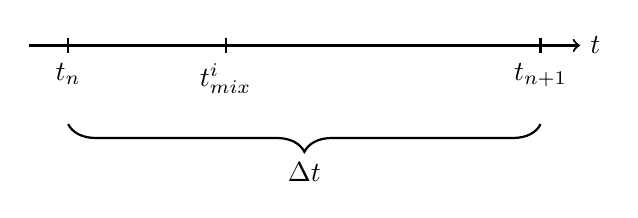
\begin{tikzpicture}[thick]

% Main timeline
\draw[->] (-0.5,0) -- (6.5,0) node[right] {$t$}; % Timeline with axis label

% Time points
\foreach \x/\label in {0/{$t_n$}, 2/{$t^i_\text{mix}$}, 6/{$t_{n+1}$}} {
    \draw (\x,0.1) -- (\x,-0.1) node[below] {\label};
}

% Braces for interval
\draw[decorate,decoration={brace,amplitude=10pt,mirror}] (0,-1) -- (6,-1) node[midway,below=10pt] {$\Delta t$};


\end{tikzpicture}
\end{figure}

arba kitaip sakant išmaišymas įvyks laiko žingsniu $t_n$, jei:

\begin{align}
    \vert t_n - t^i_\text{mix} \vert < \frac{1}{2}\Delta t \label{mix-inequality}
\end{align}

\newpage
\paragraph{Nedeterministinis maišymas}

Maišymas praktikoje yra chaotiškas procesas, todėl sudarydami kompiuterinį modelį turime į tai atsižvelgti. Maišymą modeliuosime kaip reakcijos erdvės sričių atsitiktinį išdėstymą. Pradinė erdvę $\Omega$ padalinsime į mažesnes, nepersidengiančias, vienodas kvadratines sritis $\Omega_i$, tada sugeneruosime atsitiktinę $4$-permutaciją $\sigma$ ir $4$ atsitiktinius kampus $\theta_i \in \{0, \frac{\pi}{2}, \pi, \frac{3\pi}{2}\}$. Kiekviena iš sričių $\Omega_i$ keliauja į poziciją, kurioje yra sritis $\Omega_{\sigma(i)}$, tačiau pasukta kampu $\theta_i$. 

\begin{figure}[!h]
\centering
\caption{Maišymo transformacijos pavyzdys}
\label{split-reaction-space}

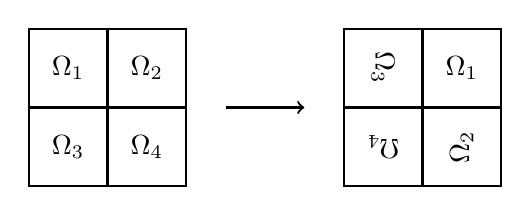
\begin{tikzpicture}
    % Original Grid
    \draw[thick] (0,0) rectangle (2,2);
    \draw[thick] (1,0) -- (1,2);
    \draw[thick] (0,1) -- (2,1);

    \node at (0.5,1.5) {$\Omega_1$};
    \node at (1.5,1.5) {$\Omega_2$};
    \node at (0.5,0.5) {$\Omega_3$};
    \node at (1.5,0.5) {$\Omega_4$};

    % Arrow
    \draw[->, thick] (2.5,1) -- (3.5,1);

    % Transformed Grid
    \begin{scope}[shift={(4,0)}]
        \draw[thick] (0,0) rectangle (2,2);
        \draw[thick] (1,0) -- (1,2);
        \draw[thick] (0,1) -- (2,1);

        \node at (0.5,1.5) {\rotatebox{270}{$\Omega_3$}}; % Rotated 180° horizontally
        \node at (1.5,1.5) {$\Omega_1$};             % No change
        \node at (0.5,0.5) {\rotatebox{180}{$\Omega_4$}}; % Upside down
        \node at (1.5,0.5) {\rotatebox{90}{$\Omega_2$}};  % 90° rotation
    \end{scope}
\end{tikzpicture}
\end{figure}


% \paragraph{Neskylančios mikrodalelės}

% Norint atkartoti praktikoje pastebimą faktą, kad išmaišymo metu reagentų mikrodalelės nėra smulkinamos, modeliuodami medžiagų maišymą apsiribojime, kad 


% aprasyti kaip tas maisymas atrodo is tikro ir kaip skiriasi nuo modelio

% matematinis modelis maisymui
% stop salyga

\subsection{Reakcijos stabdymo sąlyga}

Pristatyti kompiuterinio modelio rezultatai rodo, kad vykstant reakcijai, reagentų kiekis erdvėje artėja prie 0, tačiau niekad jo nepasiekia. Tai būdinga ir realybėje vykstančioms reakcijoms, dėl šios priežasties kompiuterinio modelio darbą stabdysime, kai sureaguos $\eta_\text{stop}\%$ pradinių medžiagų kiekio. Matematiškai reakcijos stabdymo laiką $t_\text{stop}$ galime apibrėžti taip:

\begin{align}
    q(t_\text{stop})=\left(1-\frac{\eta_\text{stop}}{100}\right)q(0),\quad \eta_\text{stop}\in[0, 100)
\end{align}

Tolimesniems pavyzdžiams ir analizei naudosime konkrečią reikšmę $\eta_\text{stop}=97$ ir reakciją stabdysime laiku $t_\text{stop}$, kai $q(t_\text{stop})=0.03q(0)$. Toks procentas pasirinktas todėl, kad sureagavus 97\% reagentų, reakcija iš esmės yra pasibaigusi ir gautų duomenų užtenka atlikti analizei.

\newpage
\subsection{Maišymo procesu papildytos programos rezultatų analizė}

\begin{figure}[h!]
\centering
\caption{Kompiuterinio modelio rezultatai - medžiagų koncentracijos per laiką, kai vyksta išmaišymas. Išmaišymo laikas $t^1_\text{mix} = 1h$ }
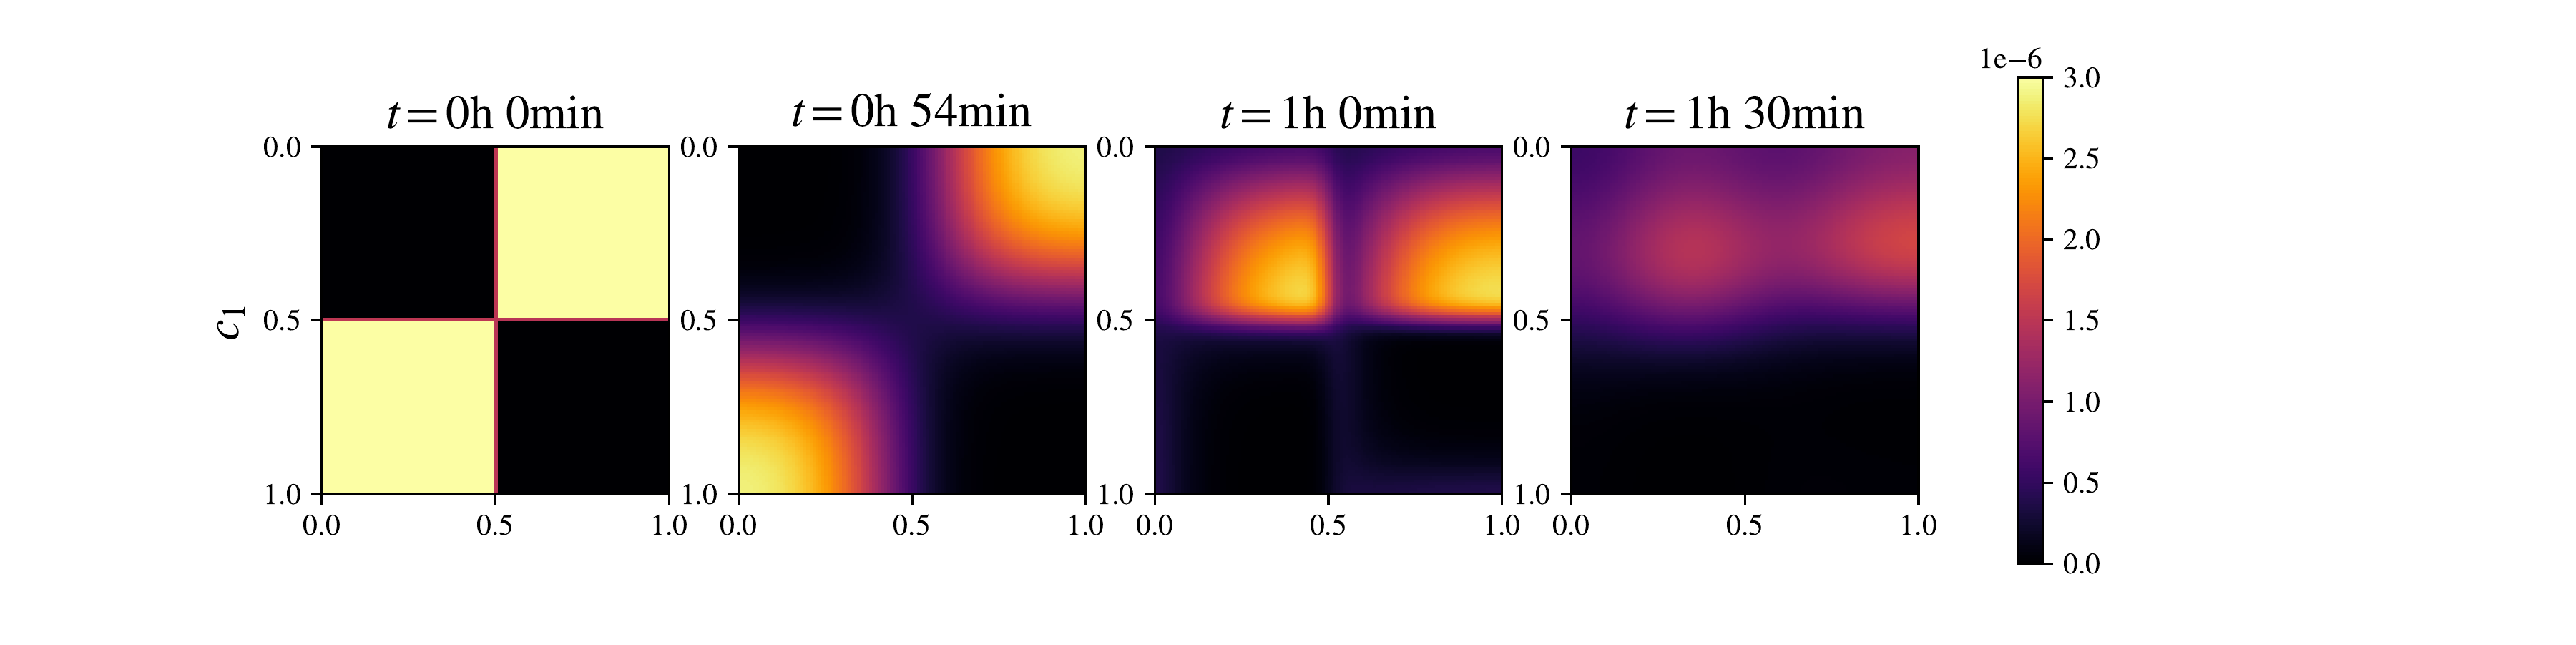
\includegraphics[width=\textwidth]{../paper/assets/random-mix-example-c0-1.png} \\
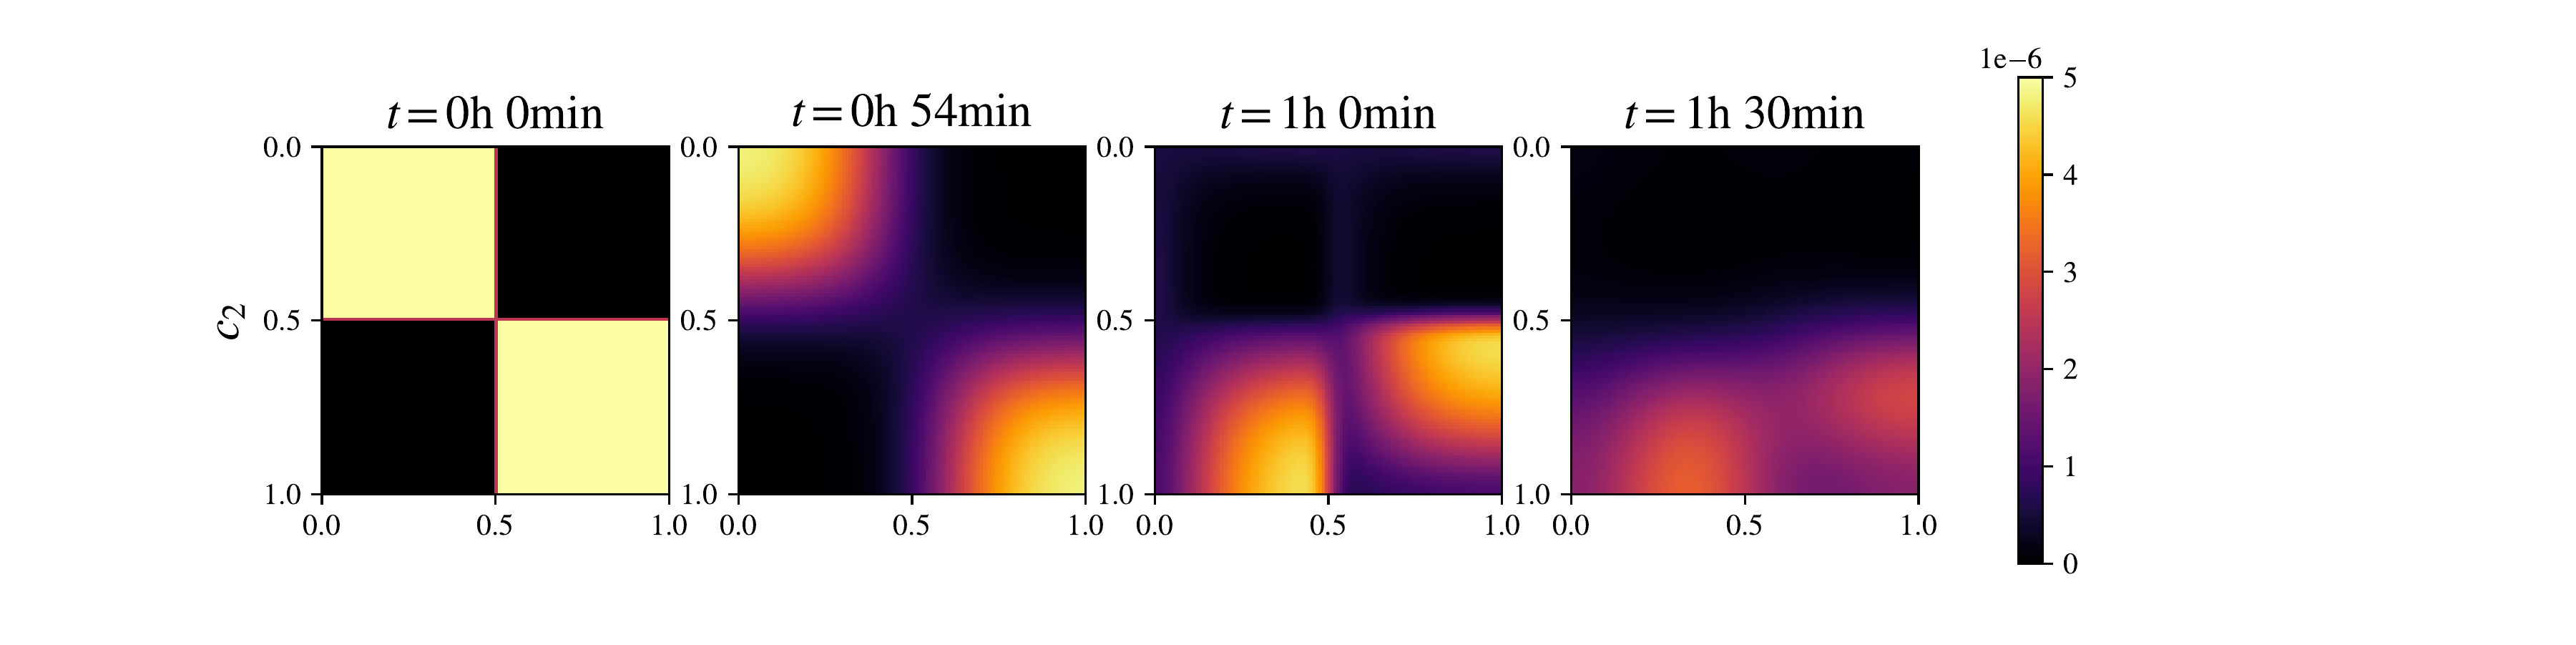
\includegraphics[width=\textwidth]{../paper/assets/random-mix-example-c1-1.png} \\
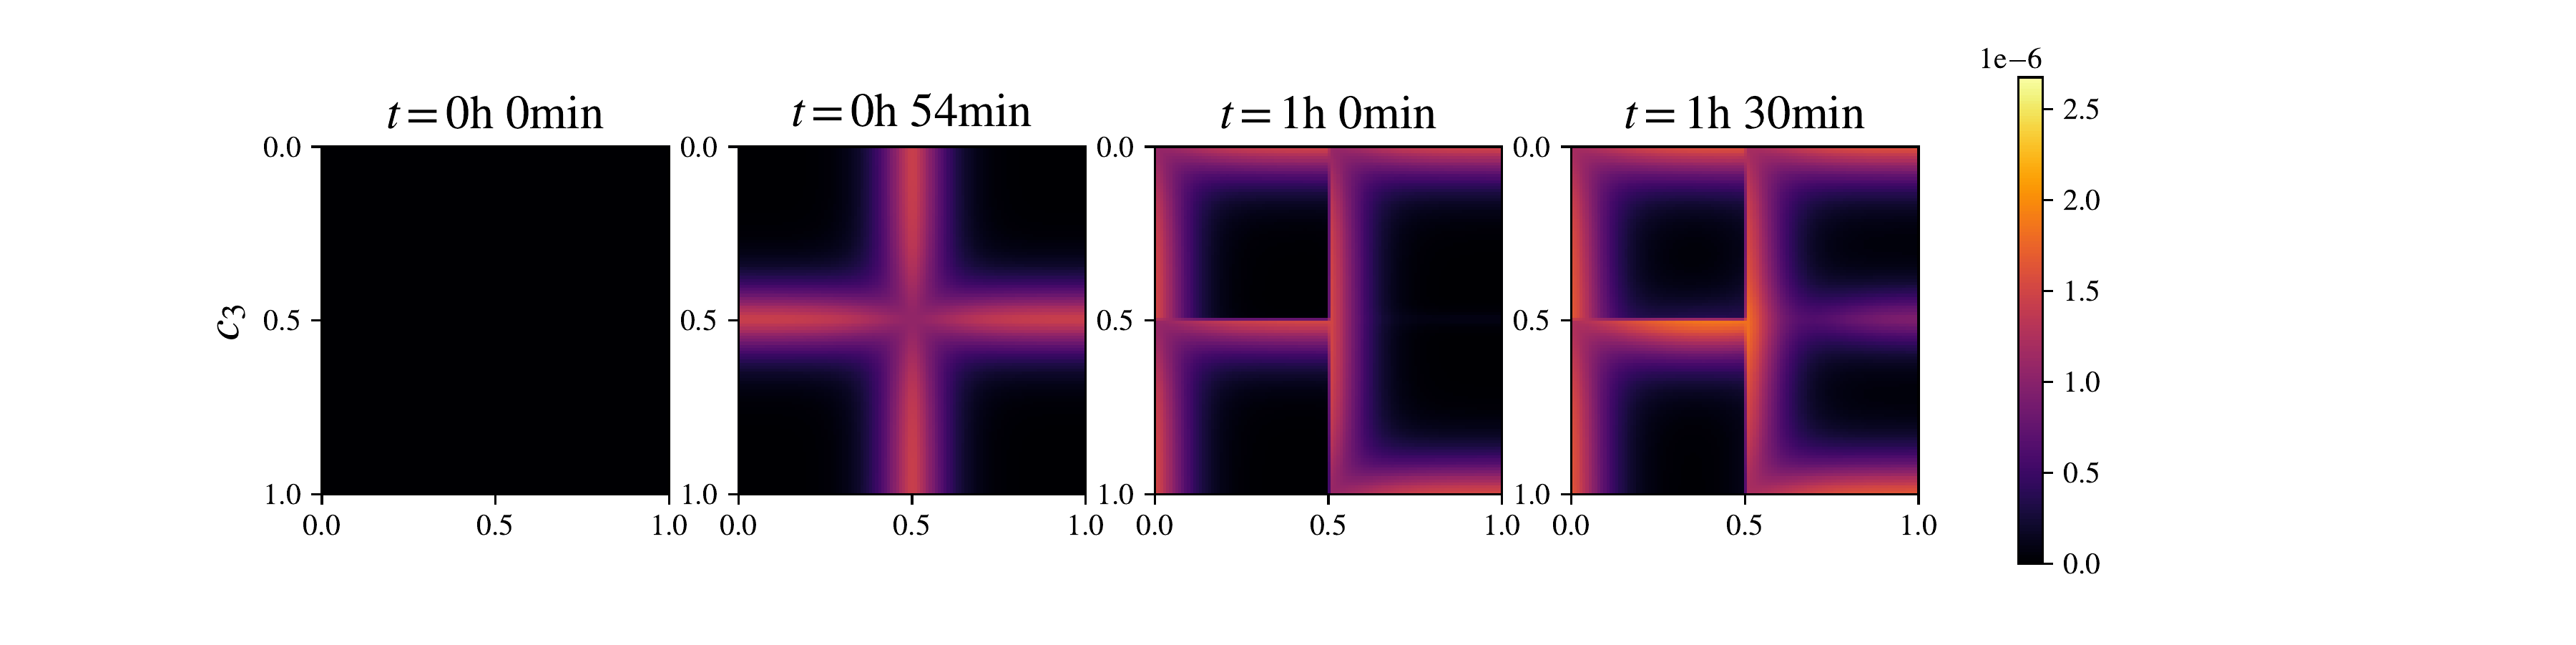
\includegraphics[width=\textwidth]{../paper/assets/random-mix-example-c2-1.png}
\label{mix-example}
\end{figure}

\ref{mix-example}-ame pavyzdyje matome kaip atrodo reakcijos eiga, kada vyksta išmaišymas. Trečiame stulpelyje ir ypatingai trečios medžiagos koncentracijoje matome ryškių artefaktų. Taip yra todėl, kad nuo išmaišymo praejo labai mažai laiko ir medžiagos nespėjo sureaguoti. Čia galime pastebėti tam tikrą problemą su atsitiktiniu išmaišymu - šiuo atveju, po išmaišymo, nesusidūrė prieš tai dar nesureagavusios dalelių kraštinės, todėl reakcijos greičiui šis procesas neturėjo beveik jokios įtakos. Tai gana akivaizdžiai matosi jei pažiūrėtume į medžiagos kiekio grafiką.

\newpage
\begin{figure}[h!]
    \centering
    \caption{Kompiuterinio modelio rezultatų palyginimas, kai išmaišymas vyksta ir nevyksta.  }
    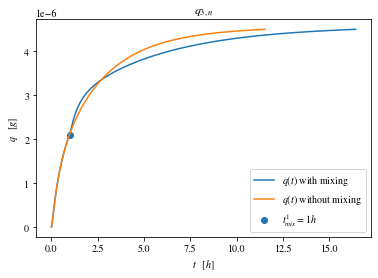
\includegraphics[width=0.5\textwidth]{../paper/assets/bad-mix-qnt-compare.png}
    \label{bad-mix-qnt-example}
\end{figure}
\ref{bad-mix-qnt-example}-ame pavyzdyje puikiai matosi, kad išmaišymas nepagreitino reakcijos, o ją sulėtino - reakcijos laikas su išmaišymu yra apytiksliai $5$-iom valandom ilgesnis. Ši problema atsiranda todėl, kad mes modeliuojame ypač mažą reakcijos erdvės sritį, kurioje susiduria tik 4 mikrodalelės, dėl to nėra daug skirtingų išdėstymų, kada viena sienele galėtų dalintis skirtingų medžiagų dalelės, prie to žinoma prisideda ir faktas, kad šis modelis yra dviejų dimensijų. Eksperimentas parodė, kad nesuveiktų ir statistinis bandymas - vidutinis atsitiktinis išmaišymas taip pat neduoda geresnių rezultatų negu reakcijos modelis be išmaišymų. Kad išspręstume šia problemą, modeliuosime tobulą teorinį išmaišymą duotoms pradinėms sąlygoms \eqref{intial-cond}.
\begin{figure}[!h]
\centering
\caption{Tobulos maišymo transformacijos pavyzdys pradinėms sąlygmos \eqref{intial-cond}}
\label{perfect-2x2-mix}
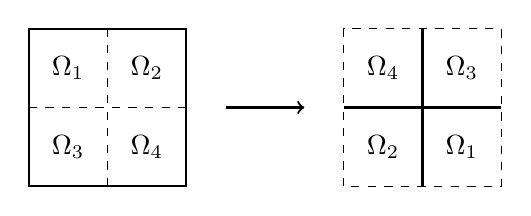
\begin{tikzpicture}
    % Original Grid
    \draw[thick] (0,0) rectangle (2,2);
    \draw[dashed] (1,0) -- (1,2);
    \draw[dashed] (0,1) -- (2,1);

    \node at (0.5,1.5) {$\Omega_1$};
    \node at (1.5,1.5) {$\Omega_2$};
    \node at (0.5,0.5) {$\Omega_3$};
    \node at (1.5,0.5) {$\Omega_4$};

    % Arrow
    \draw[->, thick] (2.5,1) -- (3.5,1);

    % Transformed Grid
    \begin{scope}[shift={(4,0)}]
        \draw[dashed] (0,0) rectangle (2,2);
        \draw[thick] (1,0) -- (1,2);
        \draw[thick] (0,1) -- (2,1);

        \node at (0.5,1.5) {$\Omega_4$};
        \node at (1.5,1.5) {$\Omega_3$};
        \node at (0.5,0.5) {$\Omega_2$};
        \node at (1.5,0.5) {$\Omega_1$};
    \end{scope}
\end{tikzpicture}
\end{figure}
\ref{perfect-2x2-mix}-ame pavyzdyje matoma prieš tai apibūdintą transformacija. Punktyrinės linijos kairėje pusėje žymi sieneles ties kuriomis vyksta reakcija. Šiuo atveju po išmaišymo nėra sričių, kurios turėtų bendrą punktyrinę sienelę, todėl šio išmaišymo dar labiau pagerinti neįmanoma. Čia geriausia išmaišymą laikome tokiu, kuris turėtų didžiausią poveiki reakcijos greičiui.
\newpage
\begin{figure}[h!]
    \centering
    \caption{Kompiuterinio modelio rezultatų palyginimas tarp įprastos reakcijos ir reakcijos su tobulu išmaišymu.  }
    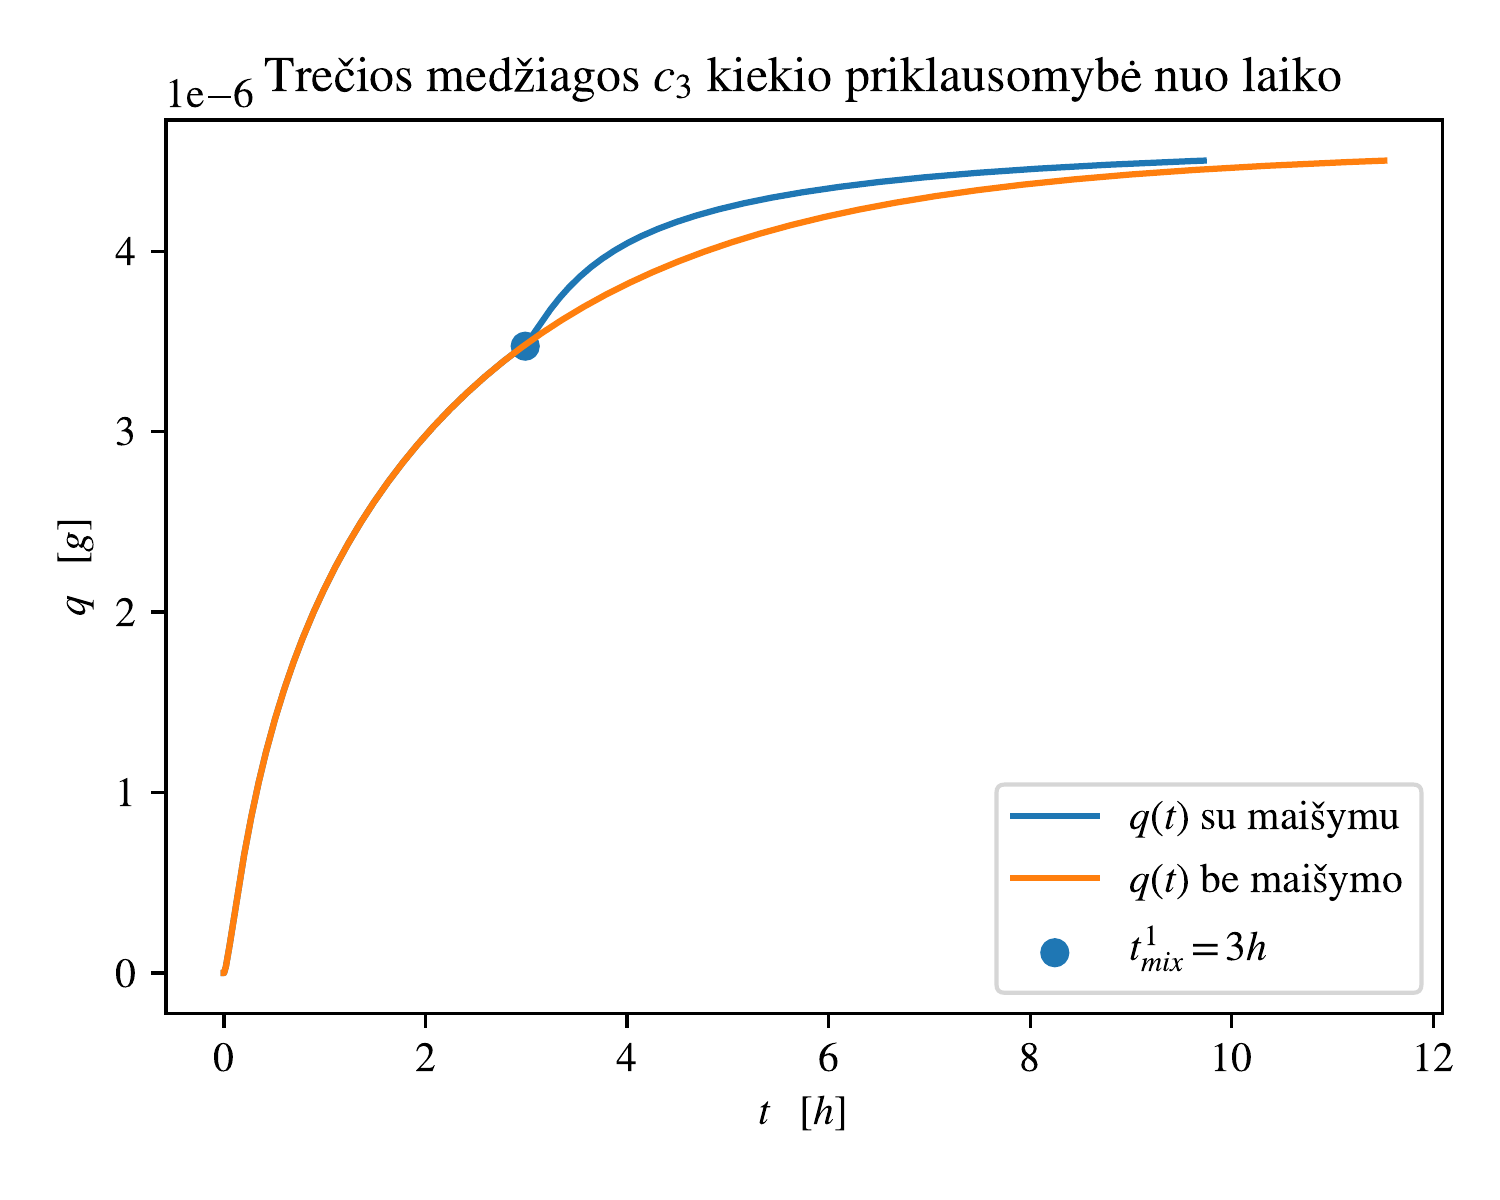
\includegraphics[width=0.5\textwidth]{../paper/assets/optimal-mix-qnt-1.png}
    \label{optimal-mix-qnt}
\end{figure}

Šiuo atveju, \ref{optimal-mix-qnt}-ame pavyzdyje matome reakcijos greičio šuolį, kuris lemia greitesnę reakcijos pabaigą. 